% This file was created by matlab2tikz.
%
%The latest updates can be retrieved from
%  http://www.mathworks.com/matlabcentral/fileexchange/22022-matlab2tikz-matlab2tikz
%where you can also make suggestions and rate matlab2tikz.
%
\definecolor{mycolor1}{rgb}{0.00000,0.44700,0.74100}%
%
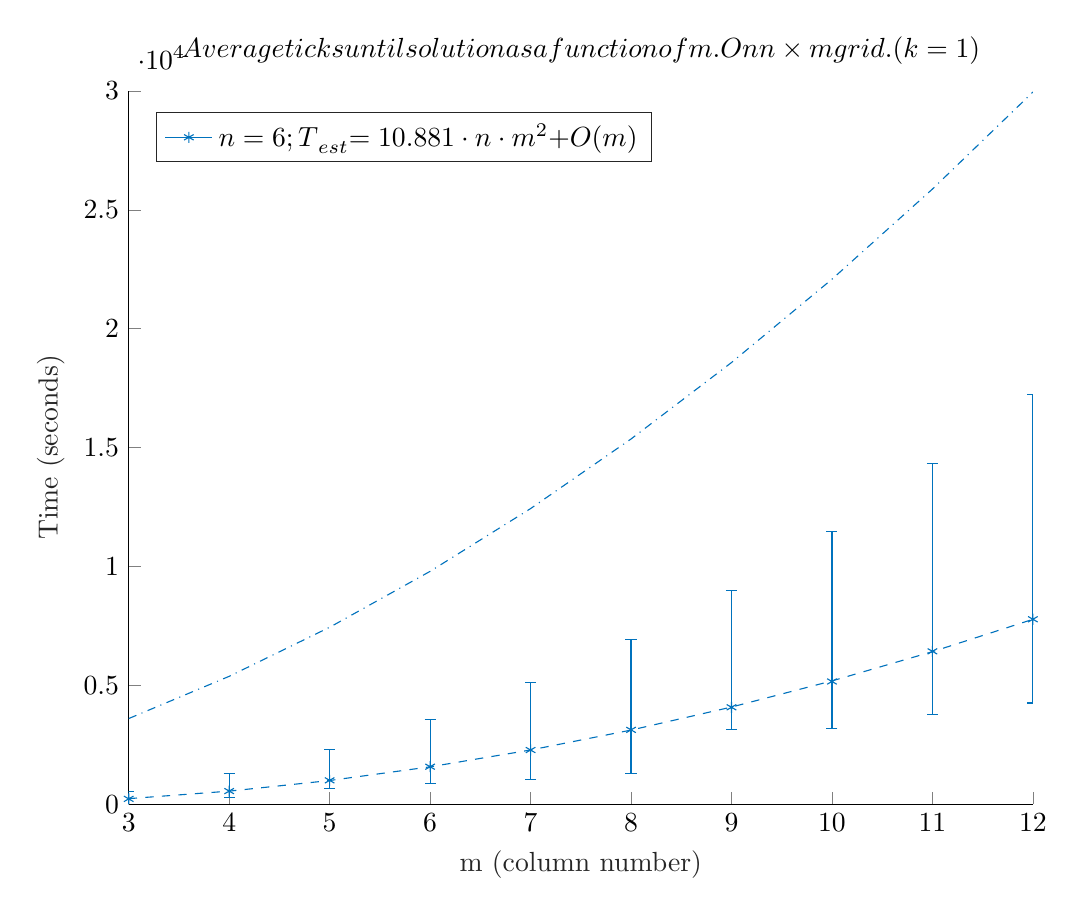
\begin{tikzpicture}

\begin{axis}[%
width=4.521in,
height=3.566in,
at={(0.758in,0.481in)},
scale only axis,
xmin=3,
xmax=12,
xlabel style={font=\color{white!15!black}},
xlabel={m (column number)},
ymin=0,
ymax=30000,
ylabel style={font=\color{white!15!black}},
ylabel={Time (seconds)},
axis background/.style={fill=white},
title style={font=\bfseries},
title={$\text{Average ticks until solution as a function of m. On n }\times\text{ m grid. (k = 1)}$},
axis x line*=bottom,
axis y line*=left,
legend style={at={(0.03,0.97)}, anchor=north west, legend cell align=left, align=left, draw=white!15!black}
]
\addplot [color=mycolor1, draw=none, mark=asterisk, mark options={solid, mycolor1}]
  table[row sep=crcr]{%
3	222.472\\
4	549.578\\
5	1001.042\\
6	1575.098\\
7	2276.66\\
8	3124.486\\
9	4074.182\\
10	5159.664\\
11	6427.76\\
12	7776.634\\
};
\addlegendentry{$\text{n = 6; T}_{\text{est}}\text{ = 10.881}\cdot\text{n}\cdot\text{m}^\text{2}\text{ + O(m)}$}

\addplot [color=mycolor1, dashdotted, forget plot]
  table[row sep=crcr]{%
3	3600\\
4	5376\\
5	7440\\
6	9792\\
7	12432\\
8	15360\\
9	18576\\
10	22080\\
11	25872\\
12	29952\\
};
\addplot [color=mycolor1, draw=none, forget plot]
 plot [error bars/.cd, y dir = both, y explicit]
 table[row sep=crcr, y error plus index=2, y error minus index=3]{%
3	222.472	324	1\\
4	549.578	742	273\\
5	1001.042	1281	345\\
6	1575.098	1997	696\\
7	2276.66	2845	1248\\
8	3124.486	3796	1844\\
9	4074.182	4920	952\\
10	5159.664	6324	1964\\
11	6427.76	7896	2660\\
12	7776.634	9456	3521\\
};
\addplot [color=mycolor1, dashed, forget plot]
  table[row sep=crcr]{%
3	231.140781818178\\
4	546.849933333331\\
5	993.136221212121\\
6	1569.99964545455\\
7	2277.44020606061\\
8	3115.4579030303\\
9	4084.05273636364\\
10	5183.22470606061\\
11	6412.97381212121\\
12	7773.30005454545\\
};
\end{axis}
\end{tikzpicture}%